\chapter{Perturbation of inputs}
\section{Methodology for perturbation}
\begin{enumerate}
    \item {Zero mean IID (Independent identical distribution) noise of certain standard deviation is added to each of the $n$ points of the graph.}
    \item {The span of points is measured for each graph and is used for scaling the Standard deviation accordingly.}
    \item {Standard deviation is scaled for each graph instead of scaling the given points in view of getting better precision in calculations.}
    \item {The algorithm is run 20 times for each experiment and the average of tour lenght was recorded.}
\end{enumerate}
\section{Results}
\subsection{Perturbation with different standard deviations}
\begin{figure}[H]
    \centering
    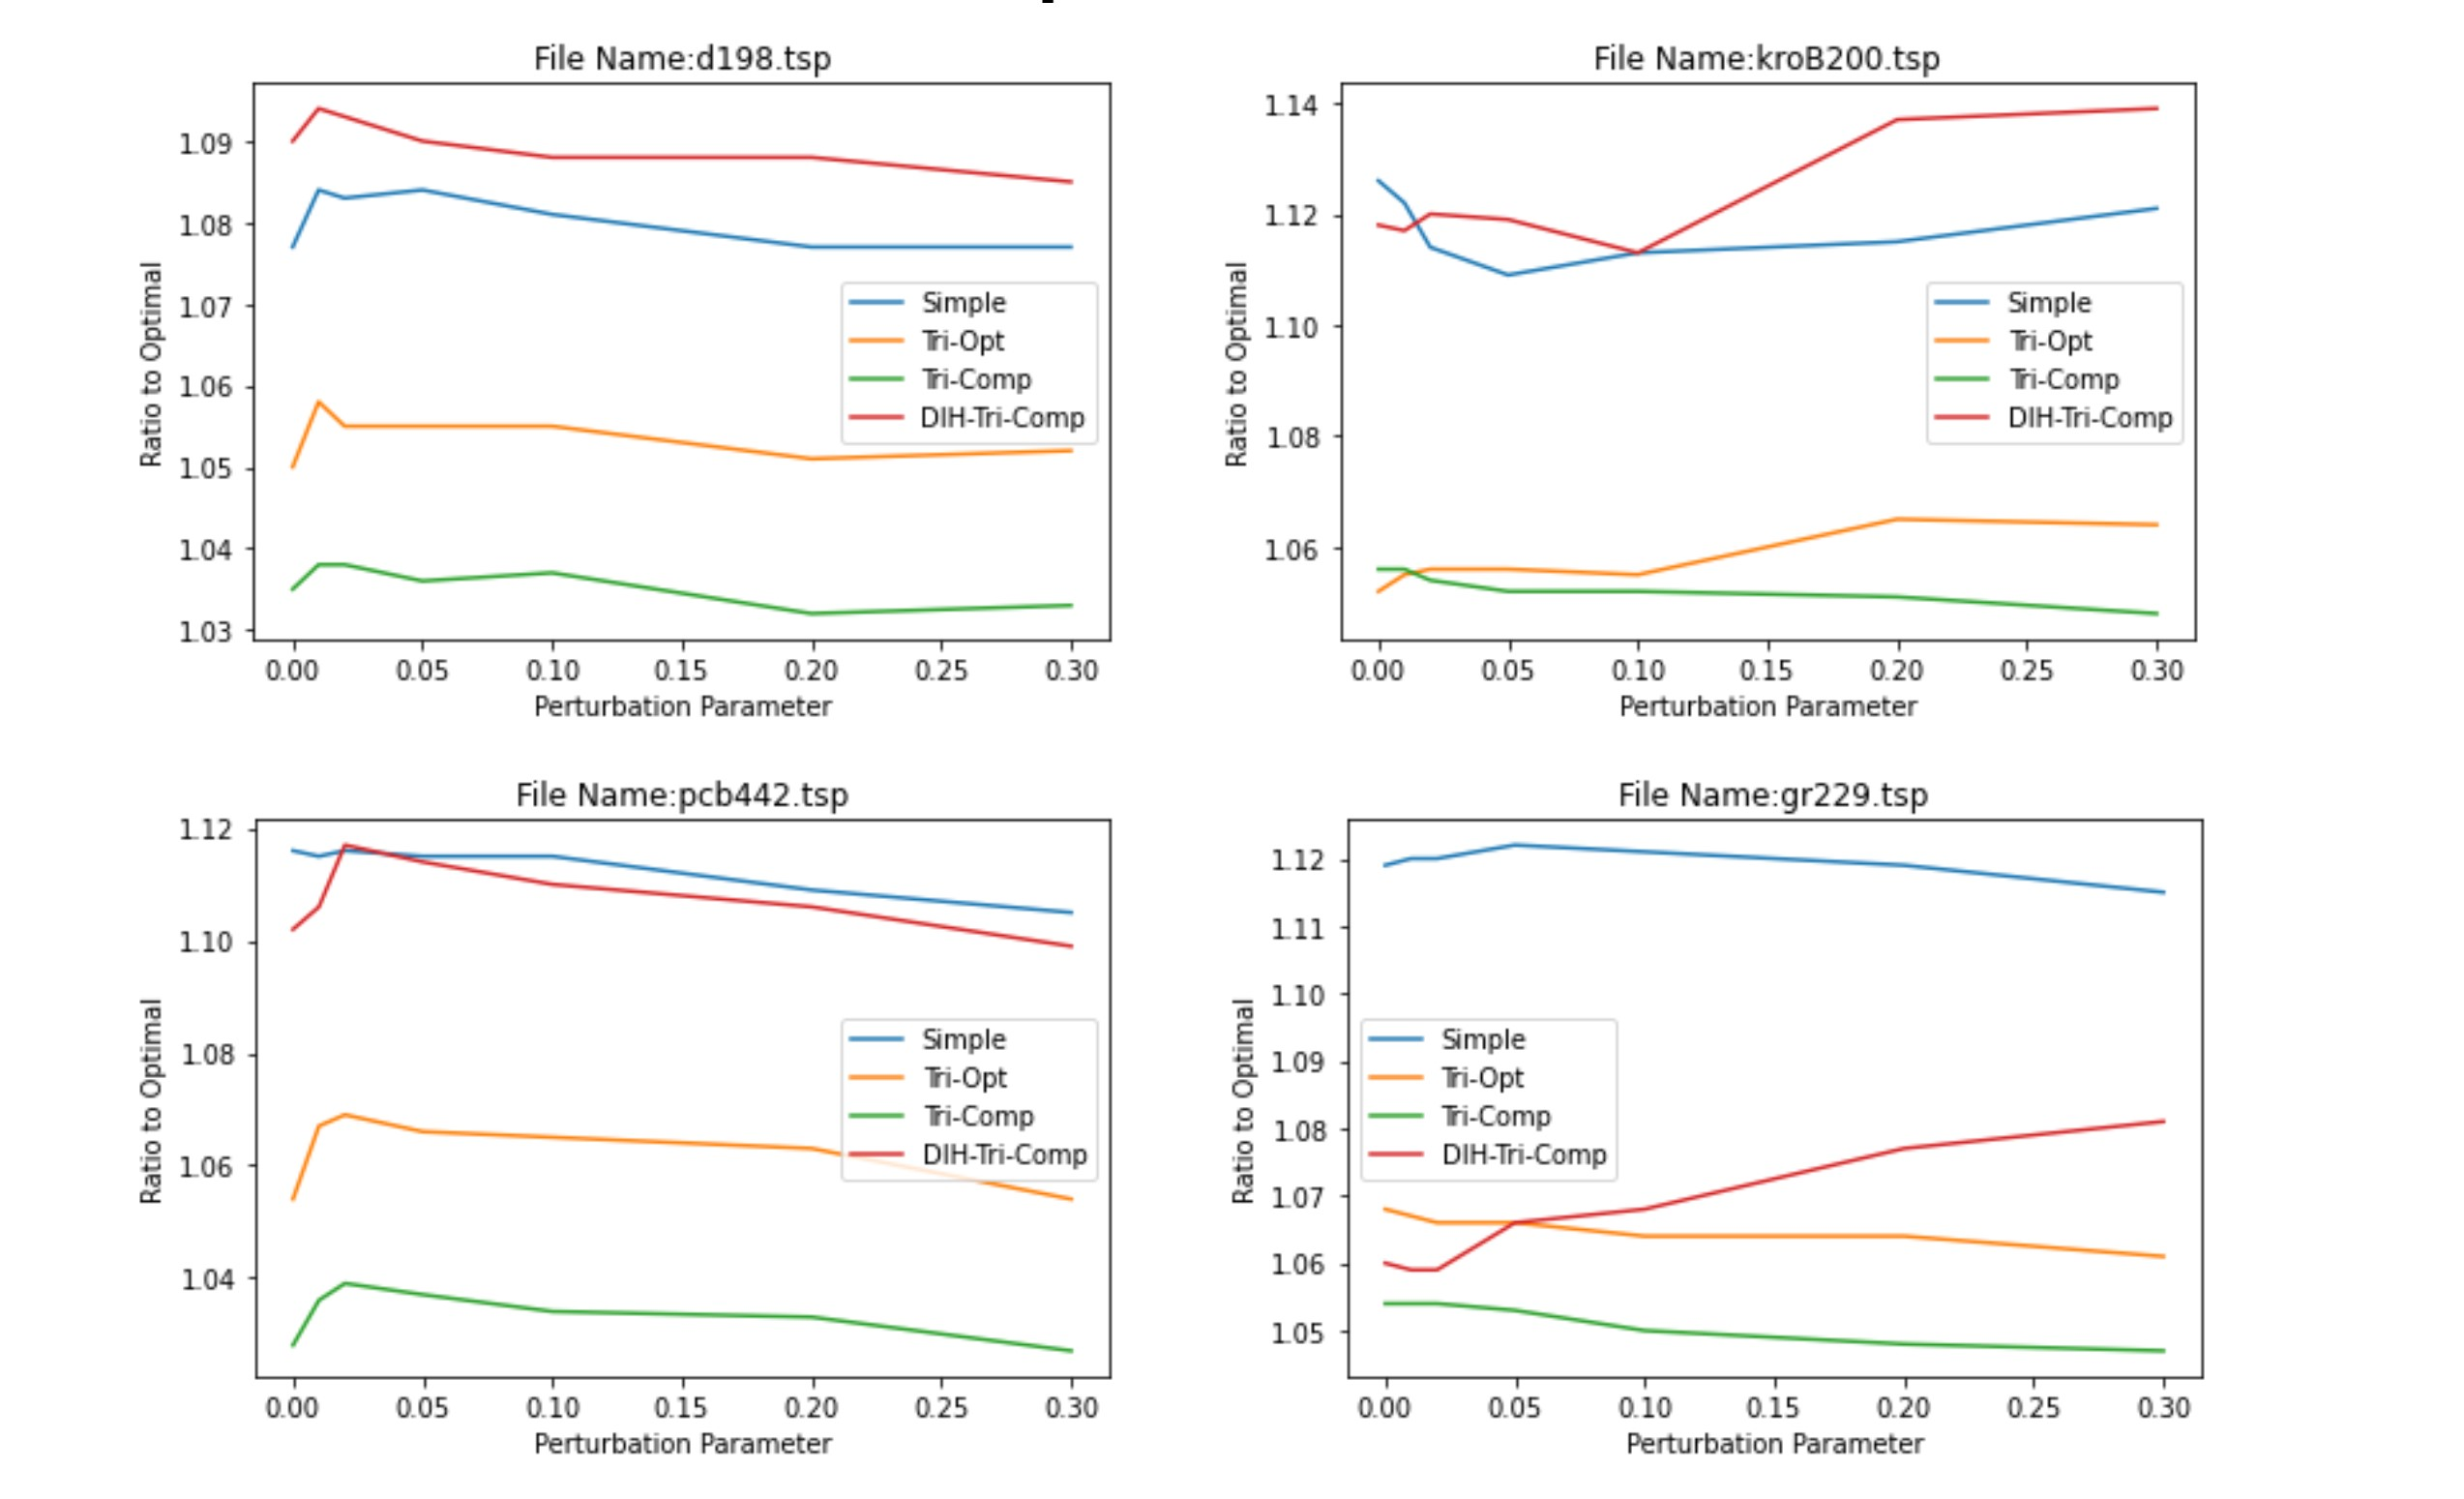
\includegraphics[scale=0.26]{7.jpg}
    \caption{Performance of heuristics on few selected datasets}
\end{figure}

\subsection{Worst case performance of heuristics on perturbation}
\begin{figure}[H]
    \centering
    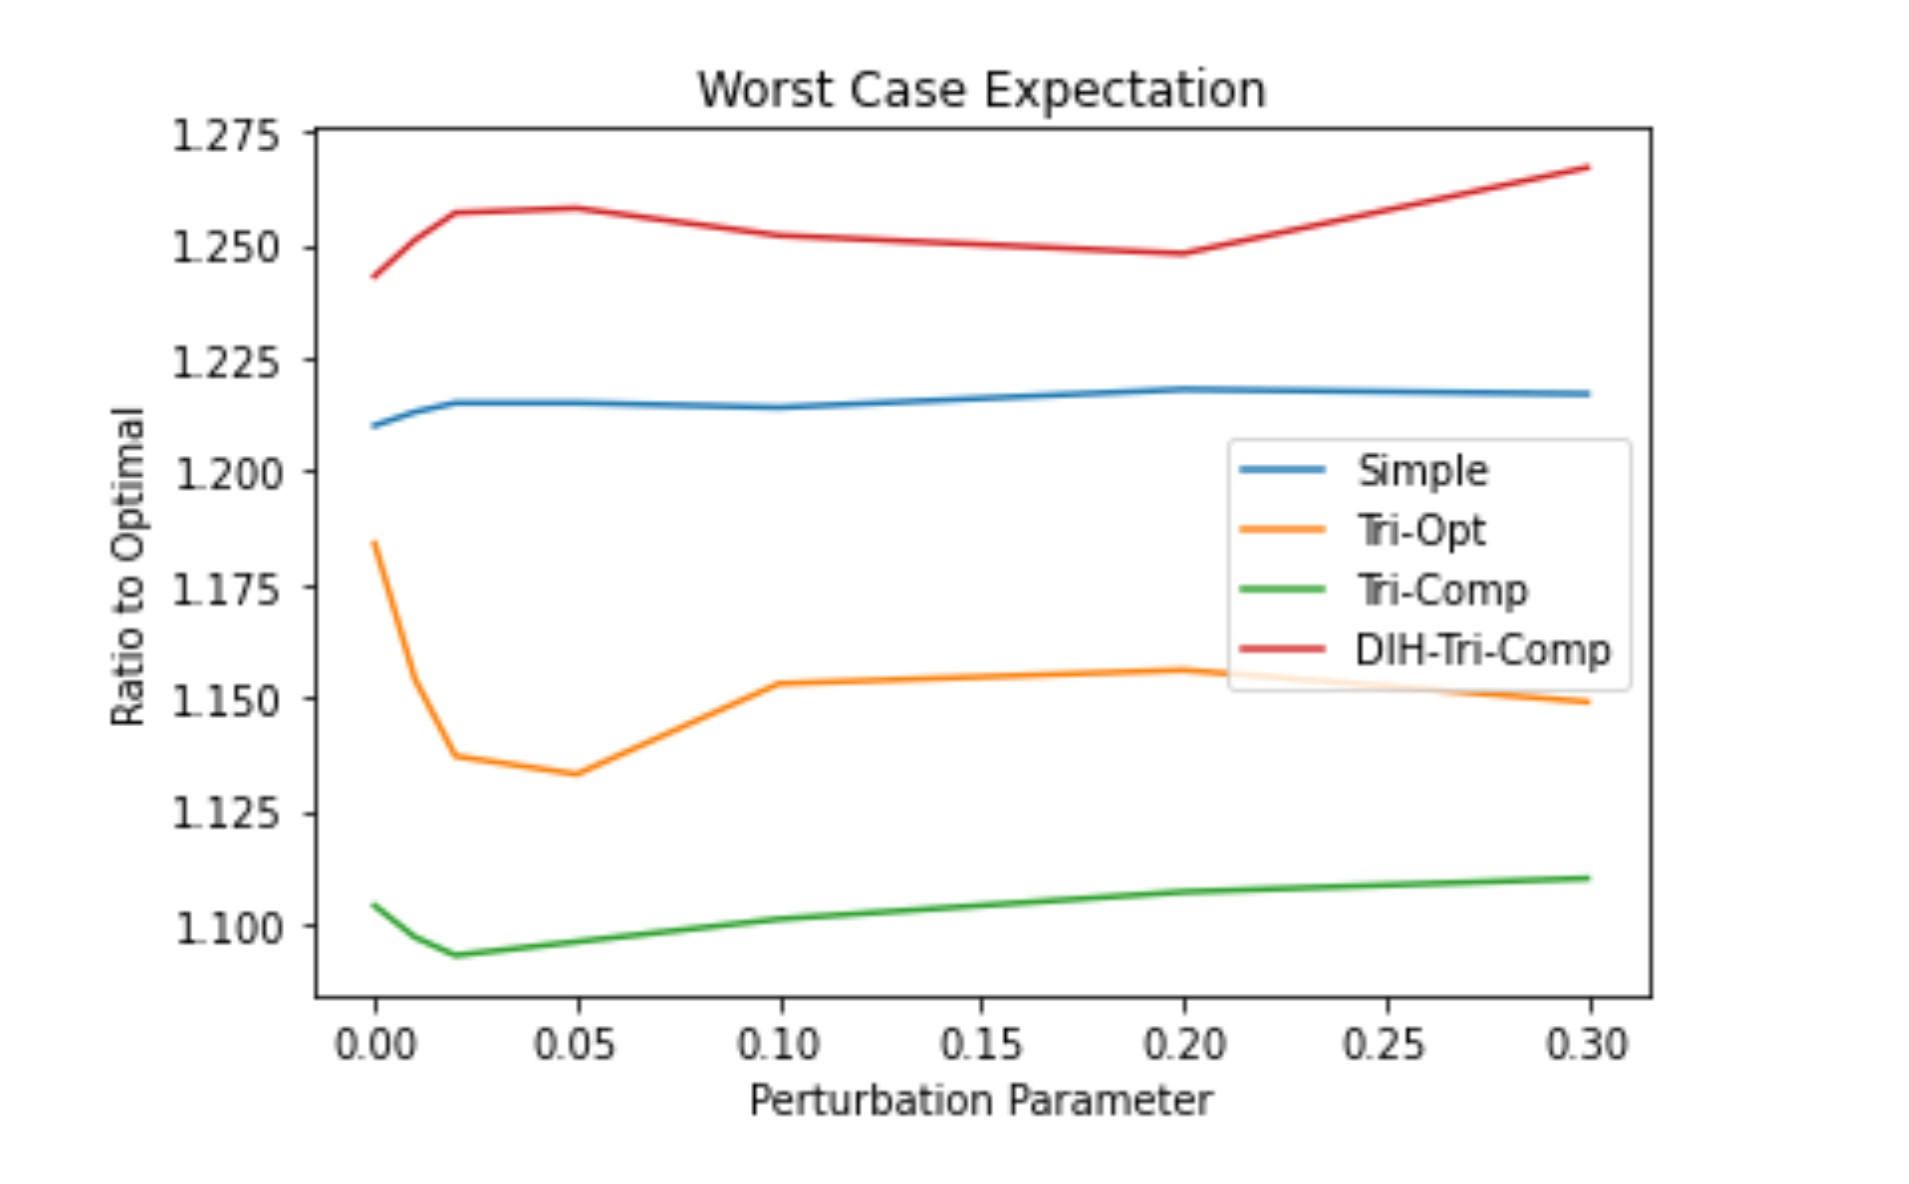
\includegraphics[scale=0.26]{8.jpg}
    \caption{Worst case performance among all files for different heuristics}
\end{figure}

\subsection{Performance of heuristics on different size graphs for each standard deviation}
\begin{figure}[H]
    \centering
    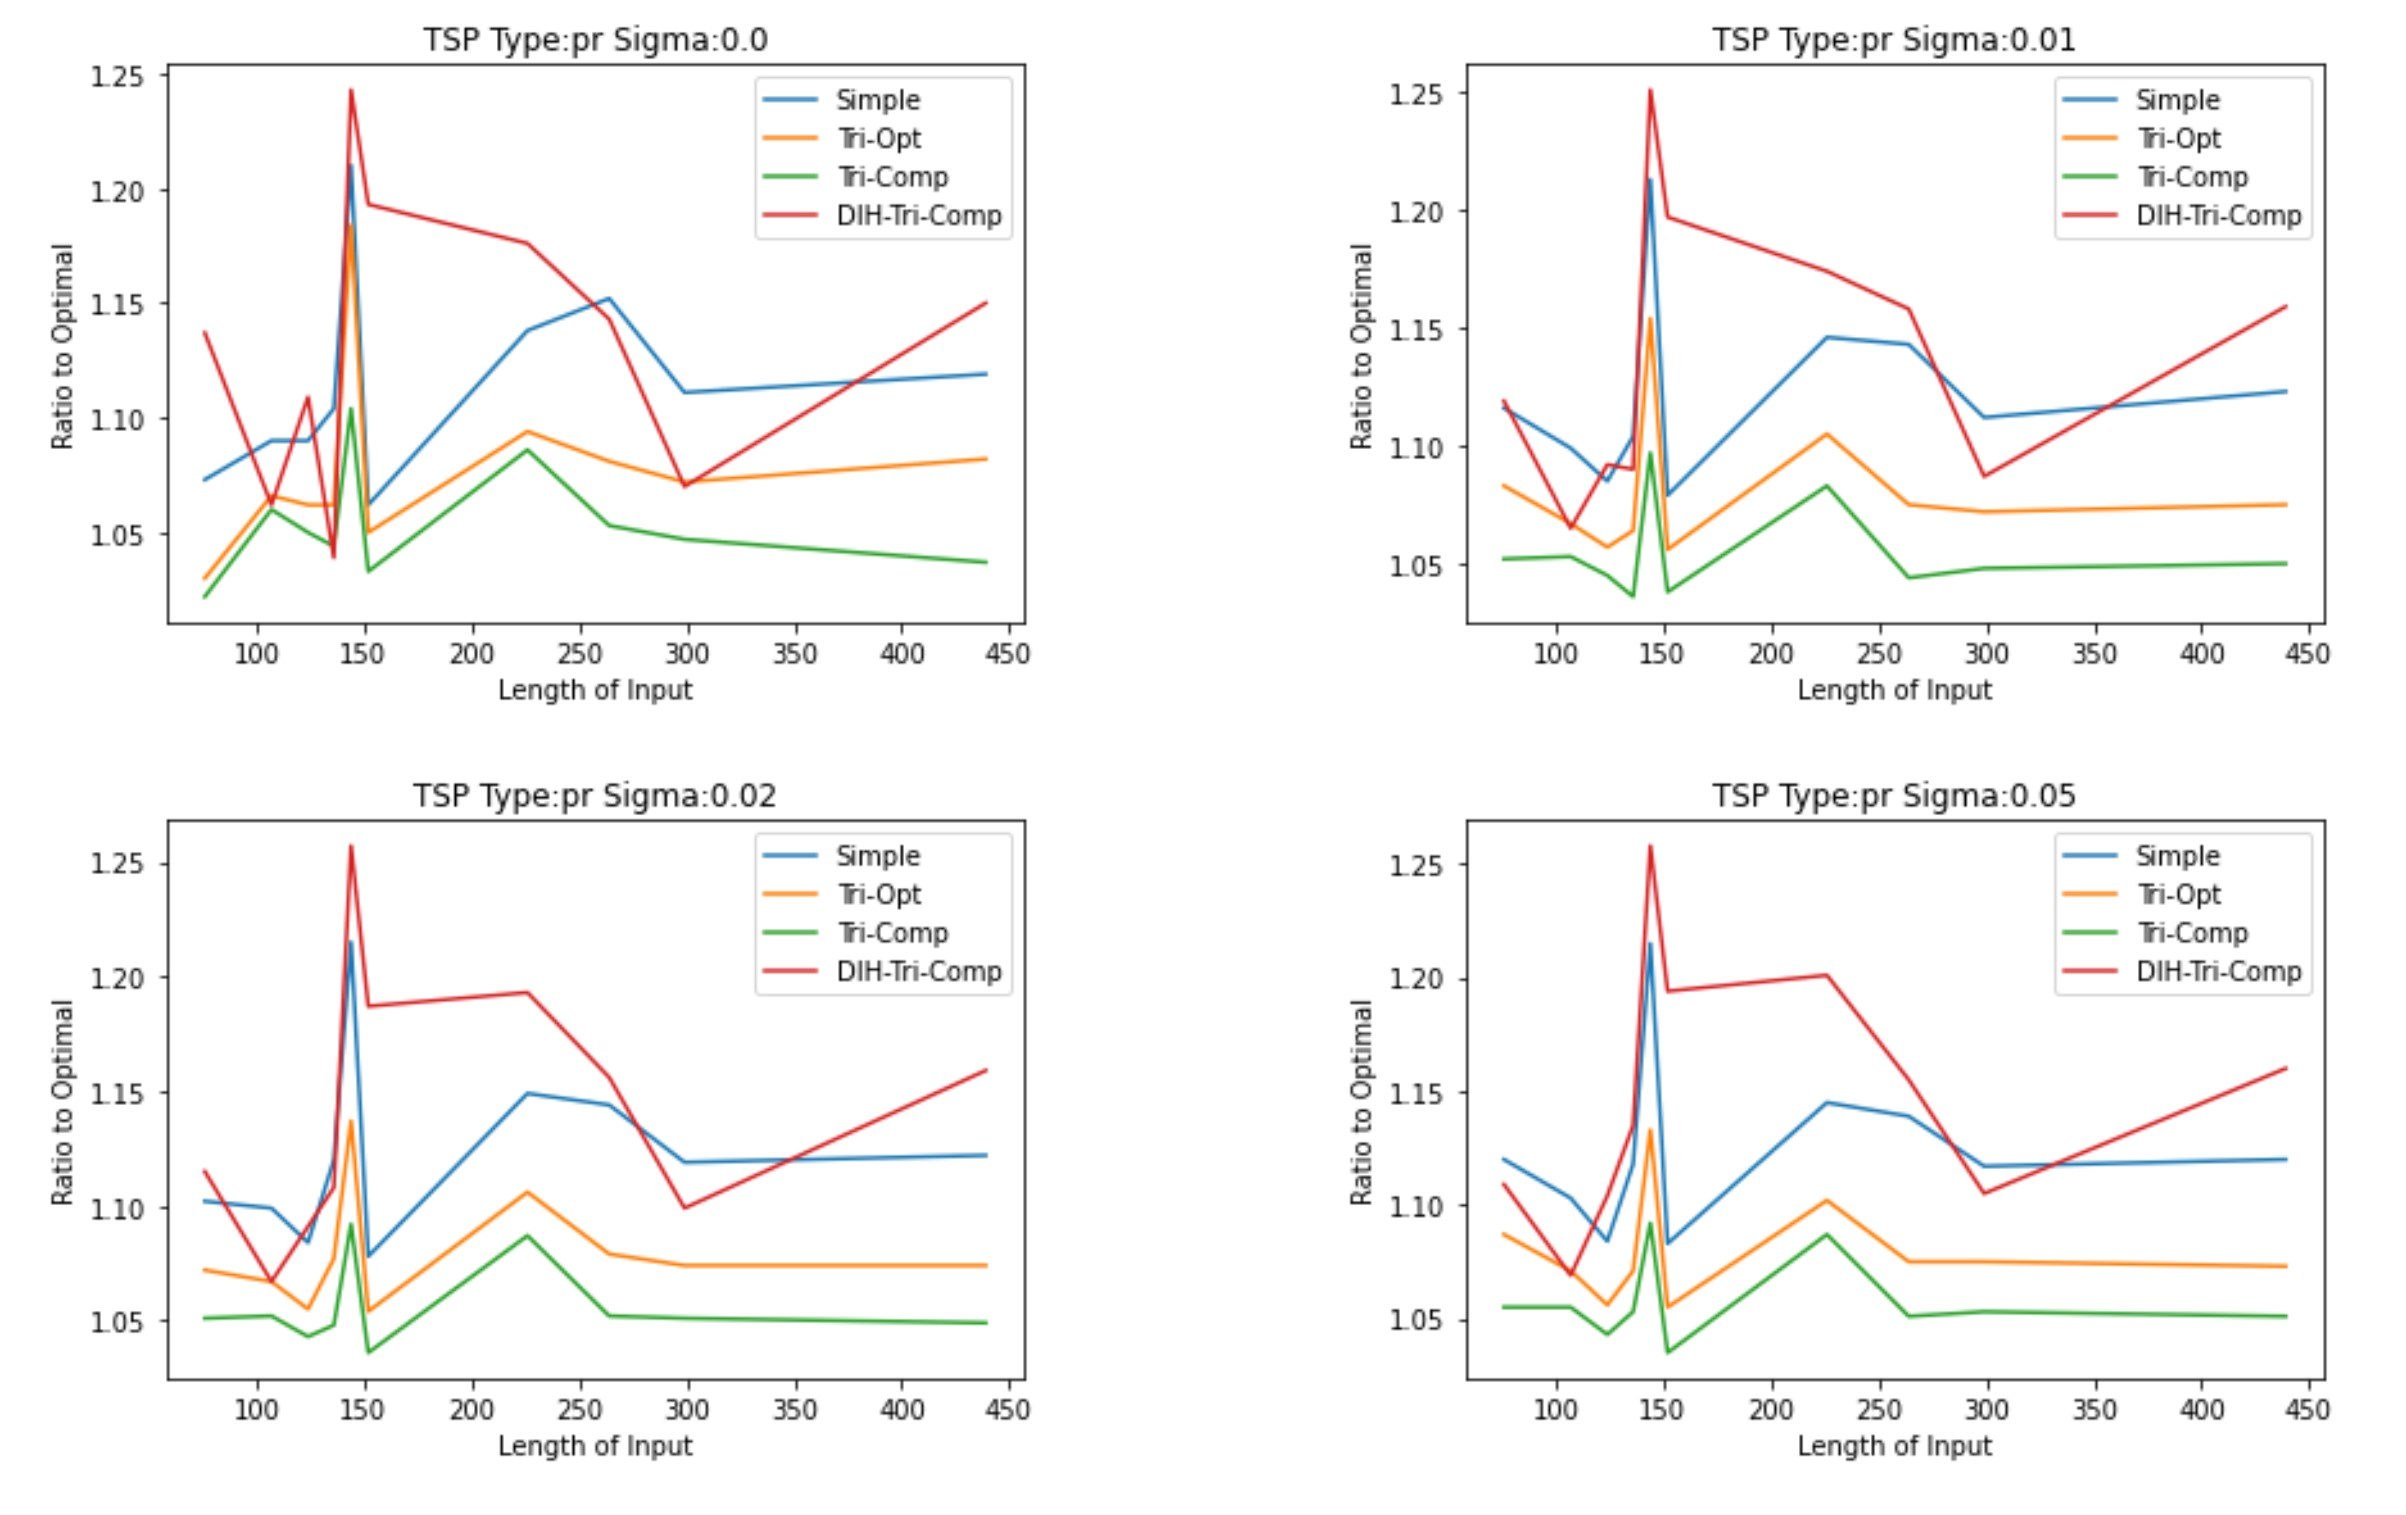
\includegraphics[scale=0.21]{9.jpg}
    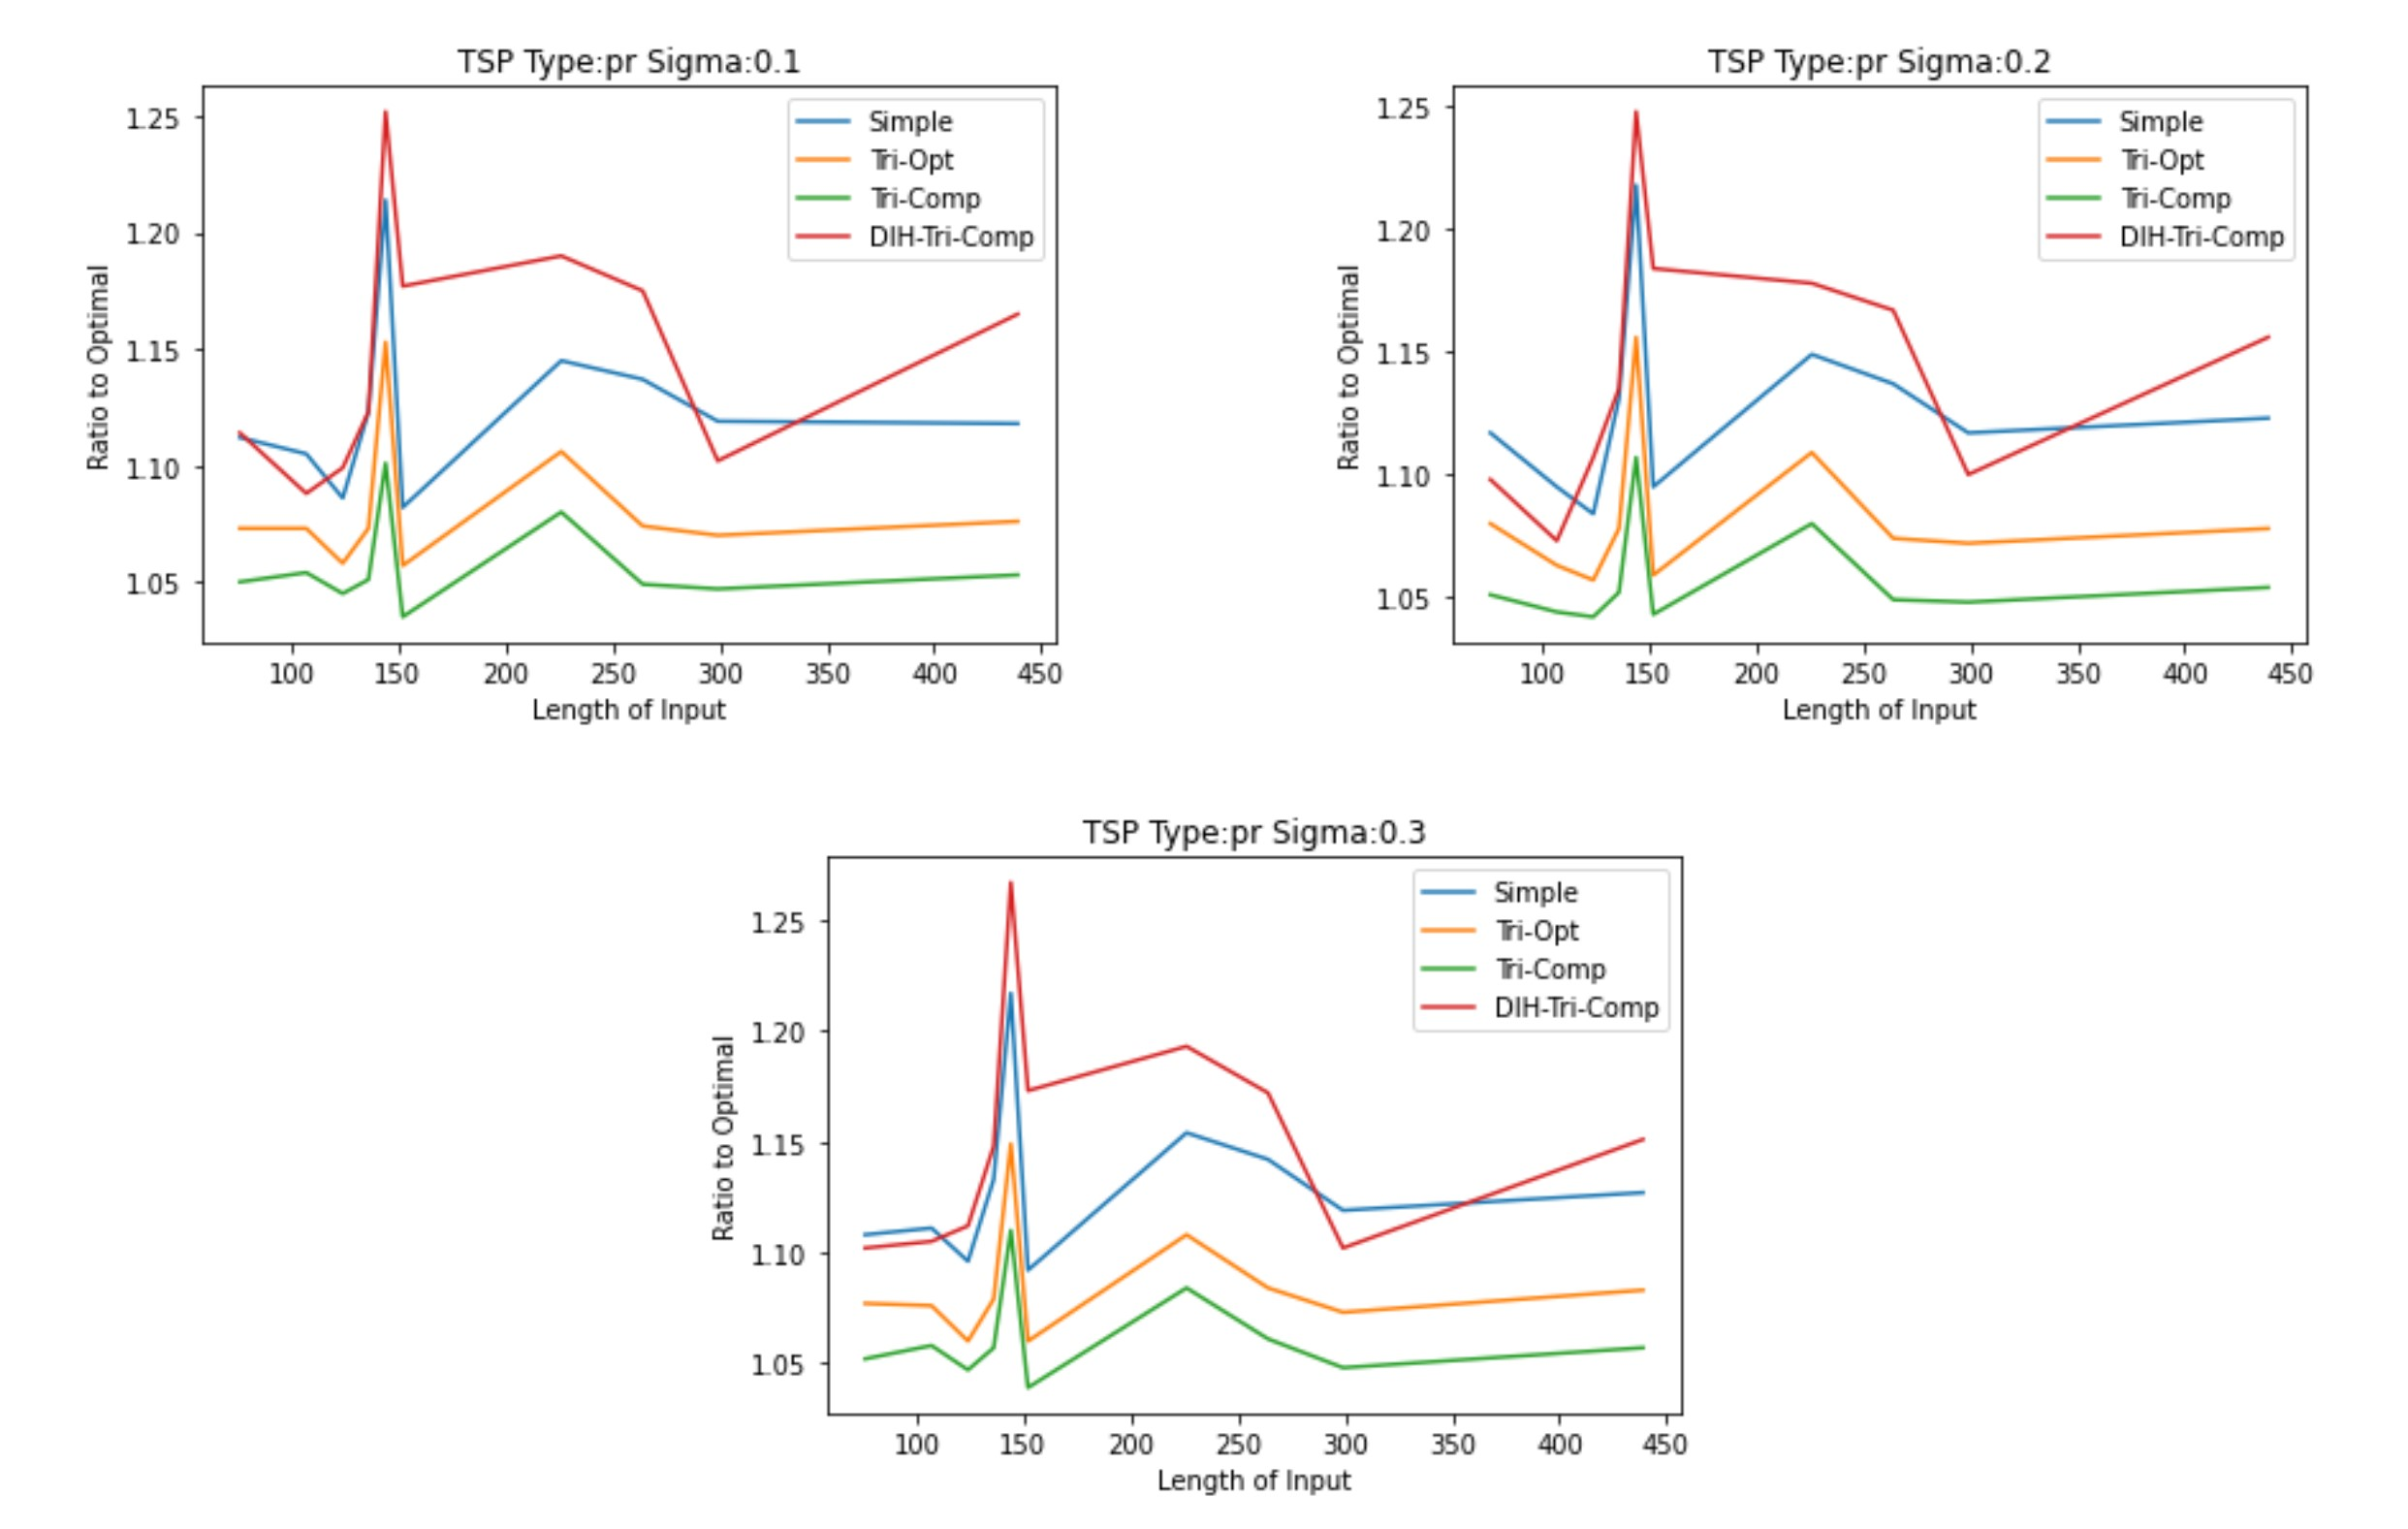
\includegraphics[scale=0.21]{10.jpg}
    \caption{Performance of heuristics on few selected datasets}
\end{figure}